\section{原始—对偶路径跟踪}
\label{sec:lpipm-path-following}

上一节得到一条曲线，但求曲线上的一个点要解一组非线性方程。于是要问：不把每个中心点算准，怎样一步步沿曲线走向$\mu=0$？做法是把三组条件当作一个方程组，同时更新$\bm{x},\bm{y},\bm{s}$。

\paragraph{主要思想：对扰动方程作Newton线性化}
当前点记为$(\bm{x},\bm{y},\bm{s})$，只要求$\bm{x},\bm{s}>\bm{0}$。为了同时适用下一节的不可行起点，这里不假设它满足等式约束。当前的平均互补量是
\begin{equation}
 \mu=\frac{\bm{x}^\top\bm{s}}{n}.
 \label{eq:lpipm-mu}
\end{equation}

我们不把目标定为$\mu=0$，而定为路径上$\sigma\mu$处的中心点，其中$\sigma\in[0,1]$称为\term{中心化参数}（centering parameter）。这一轮想达到的是
\[
 \bm{A}\bm{x}=\bm{b},\qquad\bm{A}^\top\bm{y}+\bm{s}=\bm{c},\qquad x_is_i=\sigma\mu.
\]

把新的点写成$\bm{x}+\Delta\bm{x}$、$\bm{y}+\Delta\bm{y}$、$\bm{s}+\Delta\bm{s}$，代入这三组方程。前两组本身就是线性的，第三组展开是
\[
 x_is_i+s_i\Delta x_i+x_i\Delta s_i+\Delta x_i\Delta s_i=\sigma\mu.
\]
唯一的非线性项是$\Delta x_i\Delta s_i$，它是两个小量的乘积。Newton法的做法就是把它丢掉，留下关于方向的线性方程组。

为了写得紧凑，定义三个残差，分别度量原始等式、对偶等式和互补目标还差多少：
\begin{equation}
 \bm{r}_{\mathrm{p}}=\bm{A}\bm{x}-\bm{b},\qquad
 \bm{r}_{\mathrm{d}}=\bm{A}^\top\bm{y}+\bm{s}-\bm{c},\qquad
 \bm{r}_{\mathrm{c}}=\sigma\mu\bm{1}-\bm{X}\bm{S}\bm{1},
 \label{eq:lpipm-residuals}
\end{equation}
其中$\bm{S}=\operatorname{diag}(\bm{s})$。这样，方向$(\Delta\bm{x},\Delta\bm{y},\Delta\bm{s})$由下面的线性方程组确定：
\begin{equation}
 \begin{bmatrix}
 \bm{A}&\bm{0}&\bm{0}\\
 \bm{0}&\bm{A}^\top&\bm{I}\\
 \bm{S}&\bm{0}&\bm{X}
 \end{bmatrix}
 \begin{bmatrix}\Delta\bm{x}\\\Delta\bm{y}\\\Delta\bm{s}\end{bmatrix}
 =
 \begin{bmatrix}-\bm{r}_{\mathrm{p}}\\-\bm{r}_{\mathrm{d}}\\\bm{r}_{\mathrm{c}}\end{bmatrix}.
 \label{eq:lpipm-newton}
\end{equation}
第一行要求走完之后原始残差消失，第二行要求对偶残差消失，第三行要求所有乘积都变成$\sigma\mu$。系数矩阵正是三组方程关于$(\bm{x},\bm{y},\bm{s})$的Jacobian矩阵。

\paragraph{为什么线性化$x_is_i=\mu$，而不是$s_i=\mu/x_i$}
两种写法定义同一条曲线，线性化后的方程却差别很大。图~\ref{fig:lpipm-newton-bilinear}取一个坐标，固定$s=1$、$\mu=1$，方程的根是$x=1$。图(a)对$\mu/x-s=0$作Newton法，从$x=2.4$出发，切线与横轴的交点落在$x\approx-0.96$，越过了边界。

这件事不是偶然的。$1/x$在$x$大时很平，切线斜率过小，步子迈得过大；具体地，这个迭代是$x\mapsto x(2-x)$，$x>2$时一步变成负数。图(b)对$xs-\mu=0$作Newton法，函数本身关于$x$是直线，一步到根。一般情形中$s$也在变，方程对两个变量合起来是双线性的，但误差只是一个二阶小项$\Delta x_i\Delta s_i$，线性模型“可信的范围”比倒数形式大得多。

\begin{BookInlineFigure}
  \centering
  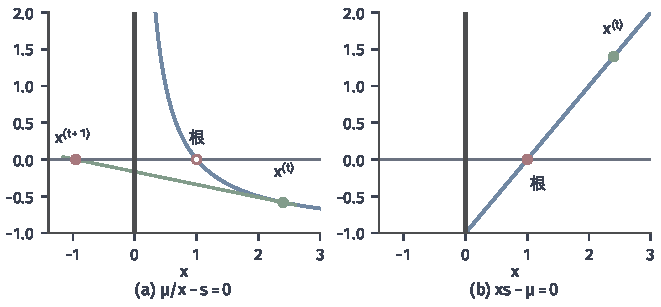
\includegraphics[width=112mm]{figures/05-optimization/01-linear-programming/matplotlib/lpipm-newton-bilinear/figure.pdf}
  \caption{同一条约束的两种写法，$s=\mu=1$，根都是$x=1$（红圈或红点）。(a)蓝线是$\mu/x-s$，绿线是在$x^{(t)}=2.4$处的切线，Newton步落到$x^{(t+1)}\approx-0.96$（红点），越过边界（深灰粗线）。(b)蓝线是$xs-\mu$，本身就是直线，Newton步一步到根。}
  \label{fig:lpipm-newton-bilinear}
\end{BookInlineFigure}

\paragraph{消元：把方程组化成一个$m\times m$的问题}
方程组~\eqref{eq:lpipm-newton}的大小是$2n+m$，但结构很特殊，可以依次消元。由第二行，
\begin{equation}
 \Delta\bm{s}=-\bm{r}_{\mathrm{d}}-\bm{A}^\top\Delta\bm{y}.
 \label{eq:lpipm-ds}
\end{equation}
第三行是$\bm{S}$与$\bm{X}$两个对角矩阵分别作用在两个方向上，直接解出
\begin{equation}
 \Delta\bm{x}=\bm{S}^{-1}\bigl(\bm{r}_{\mathrm{c}}-\bm{X}\Delta\bm{s}\bigr).
 \label{eq:lpipm-dx}
\end{equation}
把式~\eqref{eq:lpipm-ds}代入式~\eqref{eq:lpipm-dx}，得到
\[
 \Delta\bm{x}=\bm{S}^{-1}\bigl(\bm{r}_{\mathrm{c}}+\bm{X}\bm{r}_{\mathrm{d}}\bigr)+\bm{S}^{-1}\bm{X}\bm{A}^\top\Delta\bm{y}.
\]

记对角矩阵$\bm{D}=\bm{X}\bm{S}^{-1}$，它的对角元是$x_i/s_i$。把上式代入第一行$\bm{A}\Delta\bm{x}=-\bm{r}_{\mathrm{p}}$，就得到只含$\Delta\bm{y}$的方程。定义
\begin{equation}
 \bm{M}=\bm{A}\bm{D}\bm{A}^\top,\qquad
 \bm{h}=-\bm{r}_{\mathrm{p}}-\bm{A}\bm{S}^{-1}\bigl(\bm{r}_{\mathrm{c}}+\bm{X}\bm{r}_{\mathrm{d}}\bigr),
 \label{eq:lpipm-normal-data}
\end{equation}
方向$\Delta\bm{y}$由下式给出：
\begin{equation}
 \Delta\bm{y}=\bm{M}^{-1}\bm{h}.
 \label{eq:lpipm-dy}
\end{equation}
$\bm{M}\Delta\bm{y}=\bm{h}$称为\term{正规方程}（normal equations），实际计算中用Cholesky分解求解，不显式求逆。求出$\Delta\bm{y}$后，由式~\eqref{eq:lpipm-ds}得到$\Delta\bm{s}$，再由式~\eqref{eq:lpipm-dx}得到$\Delta\bm{x}$。

这一步之所以总能进行，靠的是下面的事实。

\begin{lemma}[Newton方程可解]
\label{lem:lpipm-newton-solvable}
设$\bm{A}$满行秩，$\bm{x},\bm{s}>\bm{0}$。则$\bm{M}=\bm{A}\bm{D}\bm{A}^\top$对称正定，方程组~\eqref{eq:lpipm-newton}有唯一解，由式~\eqref{eq:lpipm-dy}、\eqref{eq:lpipm-ds}、\eqref{eq:lpipm-dx}给出。
\end{lemma}

\begin{proof}
$\bm{D}$的对角元全为正。对任何$\bm{v}\neq\bm{0}$，$\bm{A}$满行秩给出$\bm{A}^\top\bm{v}\neq\bm{0}$，于是
\[
 \bm{v}^\top\bm{M}\bm{v}=(\bm{A}^\top\bm{v})^\top\bm{D}(\bm{A}^\top\bm{v})>0,
\]
所以$\bm{M}$正定。上面的消元每一步都是等价变形，故方程组的解恰好由这三个公式给出。
\end{proof}

\paragraph{一步之后三个残差怎样变}
设步长为$\alpha\in(0,1]$，$\bm{x}^+=\bm{x}+\alpha\Delta\bm{x}$，$\bm{y}^+$、$\bm{s}^+$同理。前两组方程是线性的，把第一行、第二行代入，新的残差就是
\begin{equation}
 \bm{r}_{\mathrm{p}}^+=(1-\alpha)\bm{r}_{\mathrm{p}},\qquad\bm{r}_{\mathrm{d}}^+=(1-\alpha)\bm{r}_{\mathrm{d}}.
 \label{eq:lpipm-residual-update}
\end{equation}
走完单位步（$\alpha=1$）时，等式残差恰好为零，此后一直为零。

互补量的变化由展开式得到。把$\bm{x}^+$、$\bm{s}^+$代入内积，一次项由第三行给出
\[
 \bm{s}^\top\Delta\bm{x}+\bm{x}^\top\Delta\bm{s}=\bm{1}^\top\bm{r}_{\mathrm{c}}=n\sigma\mu-n\mu,
\]
于是
\begin{equation}
 (\bm{x}^+)^\top\bm{s}^+=\bigl(1-\alpha(1-\sigma)\bigr)\bm{x}^\top\bm{s}+\alpha^2\,\Delta\bm{x}^\top\Delta\bm{s}.
 \label{eq:lpipm-comp-update}
\end{equation}
当前点严格可行时，两个等式残差为零，第一行和第二行给出
\[
 \bm{A}\Delta\bm{x}=\bm{0},\qquad\Delta\bm{s}=-\bm{A}^\top\Delta\bm{y}.
\]
所以$\Delta\bm{x}^\top\Delta\bm{s}=0$，互补量精确地按因子$1-\alpha(1-\sigma)$下降。

\paragraph{步长：到边界的比例}
Newton方向可能把某个分量推成负数，所以步长要受限。沿方向走时，每个正分量到零的距离是确定的。定义能保持非负的最大步长
\begin{equation}
 \alpha_{\max}=\min\Bigl\{\min_{\Delta x_i<0}\frac{x_i}{-\Delta x_i},\ \min_{\Delta s_i<0}\frac{s_i}{-\Delta s_i}\Bigr\},
 \label{eq:lpipm-alpha-max}
\end{equation}
没有负分量时约定$\alpha_{\max}=+\infty$。这个量和单纯形法的比值检验是同一种计算，只是后者走到恰好有一个变量为零，这里不能走到那么远，否则下一轮的$\bm{S}^{-1}$或$\bm{D}$不存在。

取一个略小于$1$的比例$\eta$，例如$0.9$或$0.995$，令
\begin{equation}
 \alpha=\min\{1,\ \eta\,\alpha_{\max}\},
 \label{eq:lpipm-alpha}
\end{equation}
这称为\term{到边界的比例规则}（fraction-to-the-boundary rule）。图~\ref{fig:lpipm-step-rule}是贯穿例第一轮的情形：六个坐标沿方向变化，其中$s_1$最先降到零，$\alpha_{\max}$由它决定。

\begin{BookInlineFigure}
  \centering
  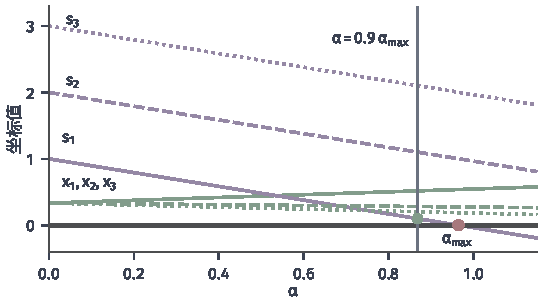
\includegraphics[width=92mm]{figures/05-optimization/01-linear-programming/matplotlib/lpipm-step-rule/figure.pdf}
  \caption{贯穿例第一轮各坐标沿Newton方向的变化，$\sigma=0.3$。紫线是$s_1,s_2,s_3$，绿线是$x_1,x_2,x_3$，实线、虚线、点线依次对应下标$1,2,3$，深灰粗线是边界。$s_1$在$\alpha_{\max}=55/57\approx0.965$处最先到达零（红点），取$\eta=0.9$后实际步长$\alpha=33/38\approx0.868$（竖线与绿点）。}
  \label{fig:lpipm-step-rule}
\end{BookInlineFigure}

\paragraph{中心化：两种力量的折中}
参数$\sigma$控制这一轮更想做什么。$\sigma=1$时目标是当前$\mu$处的中心点，方向只把点拉回路径，互补量不减；$\sigma=0$时目标直接是$\mu=0$，这个方向称为\term{仿射尺度方向}（affine-scaling direction），只求减小互补量，不管中心性。

可以把中心路径想成山谷的谷线，互补量是海拔。$\sigma=0$相当于只顾朝谷底方向走，容易撞上谷壁，步长被迫很小。$\sigma=1$相当于退回谷线，位置好了，海拔没降。合适的$\sigma$介于两者之间，类比的失效之处是，这里“谷壁”是$x_i$或$s_i$接近零的边界，不是某个目标函数的等高线。

\paragraph{计算过程}
下面把每一轮写成具体步骤，并在例~\eqref{eq:lpipm-running}上逐轮计算。取固定的中心化参数$\sigma=0.3$、比例$\eta=0.9$，容差$\varepsilon=10^{-3}$，起点选严格可行点。

\needspace{6\baselineskip}
\paragraph{变量}
\begin{itemize}
 \item $\bm{x}\in\mathbb{R}^n$：当前原始点，所有分量为正。
 \item $\bm{y}\in\mathbb{R}^m$：当前对偶变量。
 \item $\bm{s}\in\mathbb{R}^n$：当前对偶松弛，所有分量为正。
 \item $\mu$：当前平均互补量，由式~\eqref{eq:lpipm-mu}计算。
 \item $\bm{r}_{\mathrm{p}},\bm{r}_{\mathrm{d}},\bm{r}_{\mathrm{c}}$：式~\eqref{eq:lpipm-residuals}的三个残差，形状分别是$m$、$n$、$n$维。
 \item $\bm{D}$、$\bm{M}$、$\bm{h}$：对角缩放矩阵、$m\times m$的正规矩阵和右端，由式~\eqref{eq:lpipm-normal-data}计算。
 \item $\Delta\bm{x},\Delta\bm{y},\Delta\bm{s}$：本轮的方向，$\alpha_{\max},\alpha$是最大步长和实际步长。
\end{itemize}

\paragraph{初始化}
取严格可行的起点$(\bm{x}^{(0)},\bm{y}^{(0)},\bm{s}^{(0)})\in\mathcal{F}^{\circ}$，令$t=0$；起点怎样得到由下一节回答。例中取
\[
 \bm{x}^{(0)}=\Bigl(\frac13,\frac13,\frac13\Bigr)^\top,\qquad y^{(0)}=0,\qquad\bm{s}^{(0)}=(1,2,3)^\top.
\]
它满足等式约束，但不是中心点：三个乘积分别是$1/3$、$2/3$、$1$。

\needspace{6\baselineskip}
\paragraph{每轮更新}
在第$t$轮，以$(\bm{x}^{(t)},\bm{y}^{(t)},\bm{s}^{(t)})$为当前点：
\begin{enumerate}
 \item \textbf{检查停止。}按式~\eqref{eq:lpipm-residuals}计算$\bm{r}_{\mathrm{p}}$、$\bm{r}_{\mathrm{d}}$，按式~\eqref{eq:lpipm-mu}计算$\mu^{(t)}$。若等式残差和互补量都不超过容差，停止并输出当前点。

 例中第一轮
 \[
  \mu^{(0)}=\frac13\Bigl(\frac13+\frac23+1\Bigr)=\frac23,\qquad\bm{x}^\top\bm{s}=2>\varepsilon,
 \]
 等式残差都是零，继续。

 \item \textbf{计算互补残差。}按式~\eqref{eq:lpipm-residuals}计算$\bm{r}_{\mathrm{c}}$，这里的$\mu$取$\mu^{(t)}$。

 例中第一轮$\sigma\mu^{(0)}=1/5$，
 \[
  \bm{r}_{\mathrm{c}}=\frac15\bm{1}-\Bigl(\frac13,\frac23,1\Bigr)^\top=\Bigl(-\frac{2}{15},-\frac{7}{15},-\frac45\Bigr)^\top.
 \]

 \item \textbf{形成并求解正规方程。}由式~\eqref{eq:lpipm-normal-data}计算$\bm{M}$和$\bm{h}$，由式~\eqref{eq:lpipm-dy}得到$\Delta\bm{y}$。

 例中$\bm{r}_{\mathrm{p}},\bm{r}_{\mathrm{d}}$为零，$\bm{D}$的对角元是$x_i/s_i$，$\bm{A}$是一行全一，所以$\bm{M}$和$\bm{h}$都是数。第一轮
 \[
  M=\frac13+\frac16+\frac19=\frac{11}{18},\qquad h=-\sum_{i=1}^3\frac{r_{\mathrm{c},i}}{s_i}=\frac{2}{15}+\frac{7}{30}+\frac{4}{15}=\frac{19}{30},
 \]
 于是
 \[
  \Delta y=\frac{19/30}{11/18}=\frac{57}{55}\approx1.0364.
 \]

 \item \textbf{回代方向。}由式~\eqref{eq:lpipm-ds}得到$\Delta\bm{s}$，由式~\eqref{eq:lpipm-dx}得到$\Delta\bm{x}$。

 例中第一轮$\Delta\bm{s}=-\Delta y\bm{1}$，$\Delta x_i=(r_{\mathrm{c},i}-x_i\Delta s_i)/s_i$，于是
 \[
  \Delta\bm{s}=-\frac{57}{55}\bm{1},\qquad
  \Delta\bm{x}=\Bigl(\frac{7}{33},-\frac{2}{33},-\frac{5}{33}\Bigr)^\top.
 \]
 三个$\Delta x_i$相加为零，这正是$\bm{A}\Delta\bm{x}=\bm{0}$。

 \item \textbf{确定步长。}由式~\eqref{eq:lpipm-alpha-max}、\eqref{eq:lpipm-alpha}计算$\alpha_{\max}$和$\alpha$。

 例中第一轮三个$s_i$的比值分别是$\tfrac{55}{57},\tfrac{110}{57},\tfrac{165}{57}$，$x_2,x_3$的比值分别是$\tfrac{11}{2},\tfrac{11}{5}$，最小的是$s_1$的比值，所以
 \[
  \alpha_{\max}=\frac{55}{57}\approx0.9649,\qquad\alpha=\frac{9}{10}\cdot\frac{55}{57}=\frac{33}{38}\approx0.8684.
 \]

 \item \textbf{更新。}令
 \begin{equation}
  \begin{aligned}
  \bm{x}^{(t+1)}&=\bm{x}^{(t)}+\alpha\Delta\bm{x},\\
  \bm{y}^{(t+1)}&=\bm{y}^{(t)}+\alpha\Delta\bm{y},\\
  \bm{s}^{(t+1)}&=\bm{s}^{(t)}+\alpha\Delta\bm{s},
  \end{aligned}
  \label{eq:lpipm-update}
 \end{equation}
 然后令$t\leftarrow t+1$，回到第1步。这里原始变量和对偶变量用同一个步长，式~\eqref{eq:lpipm-comp-update}的精确下降公式依赖这一点。

 例中第一轮
 \[
  \bm{x}^{(1)}=\Bigl(\frac{59}{114},\frac{16}{57},\frac{23}{114}\Bigr)^\top\approx(0.5175,0.2807,0.2018)^\top,
 \]
 对偶部分是
 \[
  y^{(1)}=\frac{9}{10},\qquad\bm{s}^{(1)}=\Bigl(\frac{1}{10},\frac{11}{10},\frac{21}{10}\Bigr)^\top.
 \]
 按式~\eqref{eq:lpipm-comp-update}，互补量应是
 \[
  \Bigl(1-\frac{33}{38}\cdot\frac{7}{10}\Bigr)\cdot2=\frac{149}{190}\approx0.7842.
 \]
 直接计算$\sum_ix_i^{(1)}s_i^{(1)}$也得到这个数。

 三个乘积这时是$(0.0518,0.3088,0.4237)$，差距比起点时大了，这一步以中心性为代价换来了较长的步子。
\end{enumerate}

例中第二轮的中间量如下。当前$\mu^{(1)}=0.2614$，$\sigma\mu^{(1)}=0.07842$，
\[
 \begin{gathered}
 \bm{r}_{\mathrm{c}}=(0.0267,-0.2304,-0.3453)^\top,\\
 \bm{D}=\operatorname{diag}(5.1754,0.2552,0.0961).
 \end{gathered}
\]
第一个分量已经被压低，$x_1s_1$小于目标$\sigma\mu$，所以$r_{\mathrm{c},1}$变成正的，这一轮要把它往上拉。

正规方程给出
\[
 M=5.5267,\qquad h=0.1072,\qquad\Delta y=0.0194.
\]
回代得到
\[
 \Delta\bm{s}=-0.0194\,\bm{1},\qquad\Delta\bm{x}=(0.3670,-0.2045,-0.1625)^\top.
\]

这一轮$\alpha_{\max}=1.2412$，$0.9\alpha_{\max}>1$，所以取$\alpha=1$，于是
\[
 \begin{gathered}
 \bm{x}^{(2)}=(0.8846,0.0762,0.0392)^\top,\qquad y^{(2)}=0.9194,\\
 \bm{s}^{(2)}=(0.0806,1.0806,2.0806)^\top.
 \end{gathered}
\]
互补量精确地变为$0.3\times0.7842=0.2353$。

此后每轮都取$\alpha=1$，互补量每轮乘以$0.3$。表~\ref{tab:lpipm-run}列出全部$7$轮的中间量。第$7$轮后互补量约为$5.7\times10^{-4}$，不超过$\varepsilon$，算法停止。

\begin{BookInlineTable}
  \centering
  \footnotesize
  \begin{tabular}{@{}ccccccccc@{}}
    \toprule
    $t$ & $x_1^{(t)}$ & $x_2^{(t)}$ & $y^{(t)}$ & $\mu^{(t)}$ & $M$ & $\Delta y$ & $\alpha_{\max}$ & $\alpha$\\
    \midrule
    0 & 0.3333 & 0.3333 & 0 & 0.6667 & 0.6111 & 1.0364 & 0.9649 & 0.8684\\
    1 & 0.5175 & 0.2807 & 0.9 & 0.2614 & 5.527 & 0.0194 & 1.2412 & 1\\
    2 & 0.8846 & 0.0762 & 0.9194 & 0.0784 & 11.06 & 0.0610 & 1.3210 & 1\\
    3 & 0.9615 & 0.0261 & 0.9804 & 0.0235 & 49.12 & 0.0128 & 1.3851 & 1\\
    4 & 0.9892 & 0.0073 & 0.9932 & 0.0071 & 146.0 & 0.0047 & 1.4179 & 1\\
    5 & 0.9968 & 0.0021 & 0.9979 & 0.0021 & 477.3 & 0.0015 & 1.4247 & 1\\
    6 & 0.9990 & 0.0006 & 0.9994 & 0.0006 & 1579 & 0.0004 & 1.4274 & 1\\
    7 & 0.9997 & 0.0002 & 0.9998 & 0.0002 & & & & \\
    \bottomrule
  \end{tabular}
  \caption{贯穿例的逐轮中间量，$\sigma=0.3$、$\eta=0.9$。$x_3^{(t)}=1-x_1^{(t)}-x_2^{(t)}$，$s_i^{(t)}=c_i-y^{(t)}$。第$t$行的$M,\Delta y,\alpha_{\max},\alpha$是从第$t$个点出发那一轮的量。}
  \label{tab:lpipm-run}
\end{BookInlineTable}

最终得到
\[
 \hat{\bm{x}}\approx(0.9997,0.0002,0.0001)^\top,\qquad\hat{y}\approx0.9998,
\]
互补量约$5.7\times10^{-4}$，目标值$\bm{c}^\top\hat{\bm{x}}\approx1.0004$。由于迭代全程可行，间隙就是互补量，目标误差不超过$5.7\times10^{-4}$。实际误差约$3.8\times10^{-4}$，确实在这个界内。这里的$\hat{\bm{x}}$不是顶点，第~\ref{sec:lpipm-accuracy}节讨论这一点的影响。

\begin{BookInlineFigure}
  \centering
  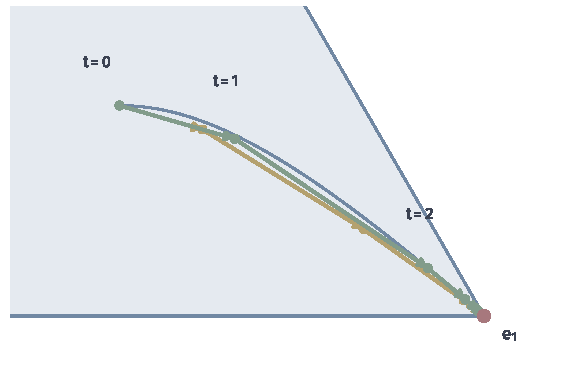
\includegraphics[width=96mm]{figures/05-optimization/01-linear-programming/matplotlib/lpipm-iterates/figure.pdf}
  \caption{贯穿例的迭代点，三角形局部放大。蓝线是中心路径，绿色是$\sigma=0.3$的路径跟踪，黄色是更激进的$\sigma=0.1$，红点是最优顶点$\bm{e}_1$。迭代点不在路径上，而是绕在路径附近前进。}
  \label{fig:lpipm-iterates}
\end{BookInlineFigure}

\paragraph{$\sigma$的取值}
图~\ref{fig:lpipm-iterates}中迭代点没有贴着路径，但始终在它附近。这种“附近”的程度可以用$\min_ix_is_i/\mu$度量，它等于$1$时点是中心点，接近$0$时某个乘积远低于平均。

图~\ref{fig:lpipm-sigma-tradeoff}比较了不同的$\sigma$。图(a)中，$\sigma$越小，互补量下降越快，但这只是因为每轮的目标更激进。图(b)说明了代价：$\sigma=0.1$前两轮的步长只有$0.63$和$0.68$，到$t=2$时中心性掉到$0.07$左右，靠后面的几轮才恢复。$\sigma=0.9$则一直很靠近中心，下降却极慢。

\begin{BookInlineFigure}
  \centering
  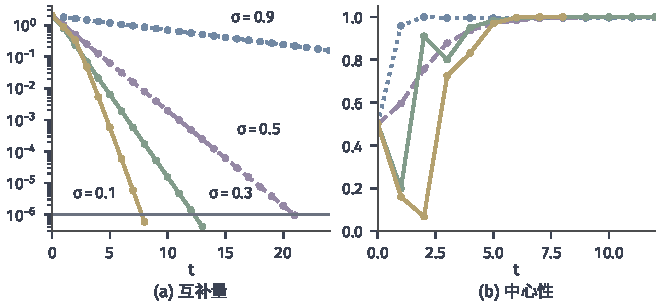
\includegraphics[width=112mm]{figures/05-optimization/01-linear-programming/matplotlib/lpipm-sigma-tradeoff/figure.pdf}
  \caption{中心化参数的影响，贯穿例，$\eta=0.9$。(a)互补量$\bm{x}^\top\bm{s}$随轮次的变化，灰色横线是$10^{-6}$。(b)中心性$\min_ix_is_i/\mu$，等于$1$表示恰好在中心路径上。绿线$\sigma=0.3$，黄线$\sigma=0.1$，紫色虚线$\sigma=0.5$，蓝色点线$\sigma=0.9$。}
  \label{fig:lpipm-sigma-tradeoff}
\end{BookInlineFigure}

\paragraph{预测—校正：先试走一步}
固定的$\sigma$有两个缺点：它不知道这一轮能走多远，也没有处理被丢掉的二阶项$\Delta x_i\Delta s_i$。\term{预测—校正}（predictor-corrector）方法用一次试算解决这两件事，额外代价只是多解一次已经分解好的方程组。

\emph{预测}是先解一次$\sigma=0$的方程组，得到仿射尺度方向$(\Delta\bm{x}^{\mathrm{a}},\Delta\bm{y}^{\mathrm{a}},\Delta\bm{s}^{\mathrm{a}})$，也就是令$\bm{r}_{\mathrm{c}}=-\bm{X}\bm{S}\bm{1}$。沿它能走的步长记为$\alpha^{\mathrm{a}}$，试走之后的平均互补量是
\begin{equation}
 \mu^{\mathrm{a}}=\frac{(\bm{x}+\alpha^{\mathrm{a}}\Delta\bm{x}^{\mathrm{a}})^\top(\bm{s}+\alpha^{\mathrm{a}}\Delta\bm{s}^{\mathrm{a}})}{n}.
 \label{eq:lpipm-mu-aff}
\end{equation}

这个数说明当前点有多好走：$\mu^{\mathrm{a}}$远小于$\mu$时，纯下降方向很有效，不需要多少中心化。常用的选法是
\begin{equation}
 \sigma=\Bigl(\frac{\mu^{\mathrm{a}}}{\mu}\Bigr)^3.
 \label{eq:lpipm-sigma-rule}
\end{equation}
三次方是一条经验规则，没有理论上的必然性。

\emph{校正}处理二阶项。式~\eqref{eq:lpipm-newton}假装$\Delta x_i\Delta s_i=0$，预测步已经给出了这一项的估计$\Delta x_i^{\mathrm{a}}\Delta s_i^{\mathrm{a}}$，于是把它移到右端：
\begin{equation}
 \bm{r}_{\mathrm{c}}=\sigma\mu\bm{1}-\bm{X}\bm{S}\bm{1}-\Delta\bm{X}^{\mathrm{a}}\Delta\bm{S}^{\mathrm{a}}\bm{1}.
 \label{eq:lpipm-corrector-rhs}
\end{equation}
用这个$\bm{r}_{\mathrm{c}}$按式~\eqref{eq:lpipm-normal-data}至\eqref{eq:lpipm-dx}求方向，步长仍按式~\eqref{eq:lpipm-alpha}。两次求解的系数矩阵$\bm{M}$相同，所以只分解一次，这一点在$\bm{M}$很大时决定了这个方法的价值。

例中第一轮，预测方向取$\sigma=0$，$M$与前面相同，右端变成$h=1$，得到
\[
 \Delta y^{\mathrm{a}}=\frac{18}{11},\qquad\Delta\bm{x}^{\mathrm{a}}=\Bigl(\frac{7}{33},-\frac{2}{33},-\frac{5}{33}\Bigr)^\top.
\]
这里$\Delta\bm{x}^{\mathrm{a}}$与固定$\sigma=0.3$时相同，是因为起点是三角形的解析中心，中心化分量在$\bm{x}$上恰好为零。

步长由$s_1$决定，试走后的互补量和中心化参数是
\[
 \alpha^{\mathrm{a}}=\frac{11}{18},\qquad\mu^{\mathrm{a}}=\frac{7}{27}\approx0.2593,\qquad\sigma=\Bigl(\frac{7}{18}\Bigr)^3\approx0.0588.
\]

校正的右端由式~\eqref{eq:lpipm-corrector-rhs}算出，其中$\sigma\mu\approx0.0392$，二阶项的估计是
\[
 \Delta\bm{X}^{\mathrm{a}}\Delta\bm{S}^{\mathrm{a}}\bm{1}\approx(-0.3471,0.0992,0.2479)^\top,
\]
于是
\[
 \bm{r}_{\mathrm{c}}\approx(0.0530,-0.7266,-1.2087)^\top,\qquad h\approx0.7132,\qquad\Delta y\approx1.1671.
\]

这一步的最大步长是$\alpha_{\max}\approx0.8568$，取$\alpha\approx0.7711$，得到
\[
 \bm{x}^{(1)}\approx(0.6742,0.2032,0.1226)^\top,\qquad y^{(1)}=0.9,\qquad\bm{x}^\top\bm{s}\approx0.5485.
\]
相比之下，固定$\sigma=0.3$第一轮后的互补量是$0.7842$。

图~\ref{fig:lpipm-predictor-corrector}(a)显示了校正的作用。黄色柱是单位预测步之后的乘积，第一个分量甚至为负，也就是说走完单位步会越界。绿色柱是校正后的单位步，三个乘积都向目标$\sigma\mu$靠拢，虽然这一轮离路径较远，并没有完全到位。

图(b)显示，整体上预测—校正用$7$轮把互补量降到$10^{-6}$以下，固定$\sigma=0.3$用$13$轮。需要说明，这是这个小例子上的观察，式~\eqref{eq:lpipm-sigma-rule}没有迭代次数的一般保证。

\begin{BookInlineFigure}
  \centering
  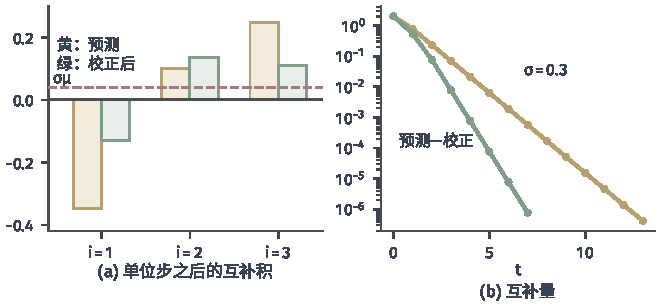
\includegraphics[width=112mm]{figures/05-optimization/01-linear-programming/matplotlib/lpipm-predictor-corrector/figure.pdf}
  \caption{预测—校正的效果，贯穿例。(a)从起点走单位步之后三个乘积$x_is_i$的值：黄色为预测方向，绿色为校正后方向，红色虚线是目标$\sigma\mu\approx0.039$。(b)互补量随轮次的变化，绿线为预测—校正，黄线为固定$\sigma=0.3$，两者都取$\eta=0.9$，容差为$10^{-6}$。}
  \label{fig:lpipm-predictor-corrector}
\end{BookInlineFigure}

\paragraph{计算代价}
每轮的主要工作是形成$\bm{M}=\bm{A}\bm{D}\bm{A}^\top$并作Cholesky分解。稠密情形下，形成$\bm{M}$需要约$m^2n$次运算，分解需要约$m^3/3$次运算；稀疏情形下取决于分解的填充，第~\ref{sec:lpipm-comparison}节再详细讨论。

$\bm{M}$的非零模式只由$\bm{A}$决定，每轮只有$\bm{D}$的数值在变，所以分解的符号结构只需分析一次。回代得到$\Delta\bm{s}$和$\Delta\bm{x}$的代价相对可以忽略。
